	\documentclass{article}
%\usepackage{lipsum}
\usepackage[utf8]{inputenc}
\usepackage[T1]{fontenc}
\usepackage{amsfonts}
\usepackage{amsmath}
\usepackage{amsthm}
\usepackage{hyperref}
\usepackage[croatian]{babel}
\usepackage{graphicx}
\title{Granice za Remzijeve brojeve i primene}
\date{15.1.2020}
\author{Mihailo Milenković, Dejan Gjer, Bojana Čakarević}

\theoremstyle{definition}
\newtheorem{definicija}{Definicija}[section]
\newtheorem{teorema}{Teorema}[section]
\newtheorem{posledica}{Posledica}[teorema]
\newtheorem{lema}[teorema]{Lema}
\newcommand{\dokaz}[1]{\begin{proof}[Dokaz]#1\end{proof}}
\begin{document}
	
	\maketitle
	
	\newpage
	
	\tableofcontents
	
	\newpage
	
	\section{Uvod}
	
	Remzijeva teorija je oblast matematike koja se bavi ulsovima pod kojim se red mora pojaviti. Najjednostavnija teorema ovog tipa jeste Dirihleov princip:
	
	\begin{definicija}
		Za prirodan broj $n>0$ definišemo 
		\[
		\underline{n}:=\{1,2,\ldots,n\}.
		\]
		Neka je dat skup $X$ i neka je $r\in \mathbb{N}\textbackslash \{0\}$.\\	
		Bojenje skupa $X$ sa $r$ boja je funkcija $\chi:X\rightarrow r$
		Podskup $Y\subseteq X$ nazivano monohromatskim (u odnosu na $\chi$), ako je
		\[
		\forall y_1,y_2:\chi(y_1)=\chi(y_2)
		\]
	\end{definicija}
	\begin{teorema}[Dirihleov Princip]
		Neka je $A$ konačan skup i neka je $0<r<|A|$.\\ Ako svaki element skupa $A$ obojimo sa jednom od datih r boja, onda su najmanje dva elementa objena istom bojom.
	\end{teorema}
	
	
	Dirihleov princip se može dodatno uopštiti u sledeće tvrđenje:
	\begin{teorema}[Uopšteni Dirihleov princip]
		Neka su dati $n,r \in \mathbb{N}$, kao i $l_1,\ldots,l_r \in \mathbb{N}\textbackslash\{0\}$, gde je
		\[
		l_1+\ldots+l_r\leq n+r-1.
		\]
		Tada za svako bojenje $\chi:\underline{n}\rightarrow\underline{r}$ postoje $i\in \underline{r}$,takvo da važi $|\chi^{-1}(i)|\geq l_i$
	\end{teorema}
	
	Dirihleov princip i uopšteni Dirihleov princip služe kao osnova za sve teoreme Remzijevog tipa.
	
	Osnovna teorema Remzijeve teorije je Remzijeva teorema za grafove:
	
	\begin{definicija}
		Za skup $X$ i prirodan broj $k>0$ definišemo
		\[
		[X]^k :=\{Y\subseteq X | \:|Y|=k\}.
		\]
		Pišemo
		\[
		n\rightarrow (l_1,\ldots,l_r)
		\]
		ako za svako bojenje $\chi:[\underline{n}]^2$ postoje $i\in \underline{r}$ i $T\subseteq \underline{n}$ sa $|T|=l_i$, takvi da je $[T]^2$ u odnosu na $\chi$ $i$-monohromatsko.	
	\end{definicija}
	\begin{teorema}[Remzijeva Teorema za obojene grafove]
		Neka $l_1,\ldots, l_r \in \mathbb{N}$. Tada postoji $n$, za koje važi
		\[
		n\rightarrow(l_1,\ldots,l_r)
		\]
	\end{teorema}
	
	\begin{definicija}
		Najmanji broj $n$ za koji važi
		\[
		n\rightarrow(l_1,l_2)
		\]
		naziva se Remzijev broj i označavamo ga sa $R(l_1,l_2)$.
	\end{definicija}
	
	Remzijeva teorema se može proširiti na hipergrafove, kao i na beskonačne grafove.
	%dopuniti sa ostalim teoremama
	
	\begin{definicija}
		Za $n \in \mathbb{N},r,k\in \mathbb{N}\textbackslash \{0\}$ i $l_1,\ldots,l_r \in \mathbb{N}$ pišemo
		\[
			n \rightarrow (l_1,\ldots,\l_r)^k,
		\]
		ako za svako bojenje $\chi:[\underline{n}]^k\rightarrow \underline{r}$, postoji $i \in \underline{r}$ i $l_i$-elementni skup $T\subseteq \underline{n}$, tako da je $[T]^k \subseteq \chi^{-1}(i)$
	\end{definicija}
	\begin{teorema}[Remzijeva Teorema za obojene hipergrafove]
		Neka $l_1,\ldots,l_r,k \in \mathbb{N}$. Tada postoji $n$, za koje važi
		\[
		n\rightarrow(l_1,\ldots,l_r)^k
		\]
	\end{teorema}

	
	\begin{teorema}[Remzijeva Teorema za beskonačne grafove]
		Neka $k,r \in \mathbb{N}\textbackslash 0$.
		\noindent
		Tada za svako bojenje $\chi:[\mathbb{N}]^k\rightarrow \underline{r}$ postoje beskonačni skup $M\subseteq \mathbb{N}$ i $i\in \underline{r}$, takvi da 
		\[
			[M]^k\subseteq \chi^{-1}(i)
		\]
	\end{teorema}

	Tačne vrednosti Remzijevih brojeva je izuzetno teško izračunati. Poznato je $R(l_1,1)= (1,l_2) = 1$ i $R(l_1,2)= (2,l_2) = l$, ali za $l_1,l_2 \geq 2$ je poznato samo 9  tačnih vrednosti Remzijevih brojeva. Poznata su razna ograničenja koja važe u opštem slučaju, dok su bolja ograničenja poznata samo za neke od vrednosti $l_1\leq 10, l_2\leq 15$.
	
	\begin{figure}[h]
		\centering
		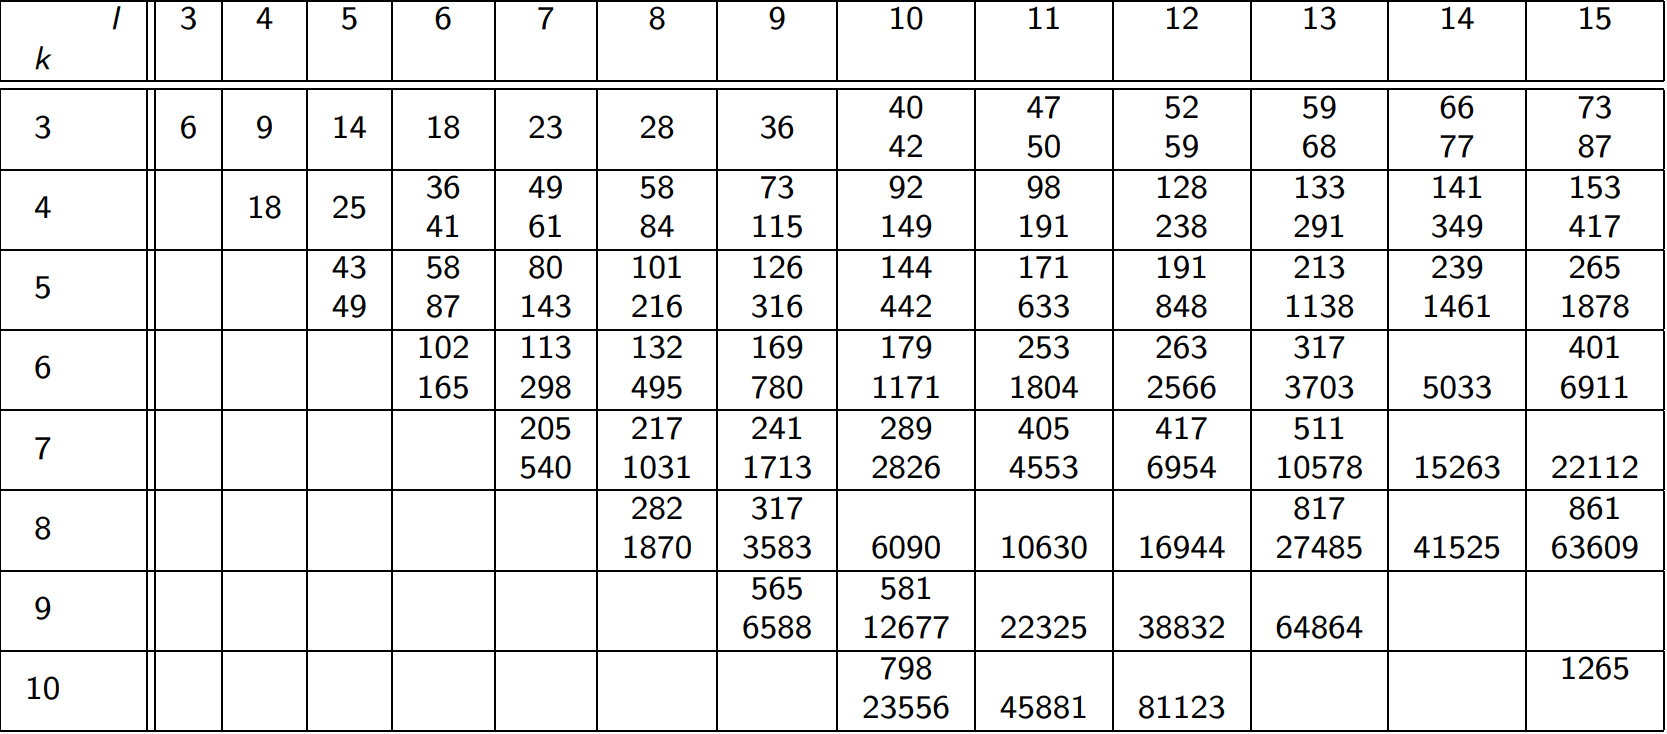
\includegraphics[width=\textwidth]{remziTabela}
		\caption{Poznate vrednosti i ograničenja Remzijevih brojeva\label{poznatiBrojevi}}
	\end{figure}
	
		%\begin{table}[h]
		%\centering
		%\begin{tabular}{|c|c|c|c|c|c|c|}
		%	$R(l_1,l_2)$   &  1 & 2 & 3 & 4 & 5 & 6\\
		%	\hline
		%	1  & 1 & 1 & 1 &  1 & 1 & 1 \\
		%	\hline
		%	2 & 1 & 2 & 3 &4 & 5 & 6\\
		%	\hline
		%	3 & 1 & 3 & 6 & 9 & 14 & 18 \\
		%	\hline
		%	4 & 1 & 4 & 9 & 18 & ? & ?\\
		%	\hline
		%	5 & 1 & 5 & 14 & ? & ? & ?\\
		%	\hline
		%	6 & 1 & 6 & 18 & ? & ? & ?\\
		%	\hline
		%\end{tabular}
		%\caption{Poznate vrednosi Remzijevih brojeva}
	%\end{table}
	
	
	Iako je poznat samo mai broj tačnih vrednosti Remzijevih brojeva, postoje mnoge teoreme u vezi ograničenja za Remzijeve brojeve. 
	
	U ovom radu ćemo prvo navesti neke od teorema u vezi gornjih ograničenja za Remzijeve brojeve (brojeva $U$, $R(l_1,l_2)\leq U$), zatim neke od teorema u vezi donjih ograničenja (brojeva $L$, $L \leq R(l_1,l_2)$). Na kraju ćemo videti neke od primena Remzijeve teoreme i njenih uopštenja u rešavanju raznih problema.
	
	
	
	\newpage
	%ako mislite da nešto nije dobro ili se treba prepraviti, označite
	\section{Gornja ograničenja za Remzijeve brojeve}
	
	\begin{teorema}
		Dirihleov opšti princip govori o tome da ako su dati $n,k \in \mathbb{N} \setminus \{0\}$ gde je $l_1+ l_2, \ldots , + l_k \leq n+k-1$, za svako bojenje $\varphi : n \rightarrow r$ postoji $i \in k$, takvo da važi $|\varphi^{-1} \geq l_i|$.
	\end{teorema}
	\dokaz{
		\[
		n,k \in \mathbb{N} \setminus \{0\}
		\]
		\[
		l_1, l_2,\ldots , l_k \in \mathbb{N} \setminus \{0\}
		\]
		\[
		l_1, l_2, \ldots , l_k \leq n+k-1
		\]
		Iz ovoga sledi $ \forall \varphi : (1,2,\ldots,n) \rightarrow (1,2,\ldots, k)(\exists i)(| \varphi^{-1}(i) \geq l_i|) $. Ako pretpostavimo suprotno, odnosno da ovo važi za svako $i$ dobijamo izraz:
		\[
		l_i \geq |\varphi^{-1}(i)|+1
		\]
		\[
		\sum\limits_{i=1}^{k} l_i \geq n+k
		\]
		Sada bi trebalo da sledi $n+k > n+k-1$ što je kontradikcija. Time je Dirihleov princip dokazan.
	}
	
	
	
	\begin{teorema}
		\[
		R(l_1,l_2) \leq R(l_2-1, l_1) + R(l_2, l_1-1)
		\]
	\end{teorema}
	\dokaz{
		Iz (...) znamo da $R(2,l_1)=l_1$ i $R(2,l_2)=l_2$. Koristeći induciju potvrđujemo da ovo važi i za svako $t$ i $s$ takvo da $t\leq l_2$ i $s<l_2$ ili $s\leq l_1$ i $t<l_2$.
		
		Pretpostavimo sada suprotno, tj. da važi tvrđenje $R(l_1,l_2) \geq R(l_2-1, l_1) + R(l_2, l_1-1)$, odnosno da postoji graf sa $R(l_1,l_2)$ čvorova koji ne sadrži podgraf izomorfan sa $K_{l_2}$ niti podgraf izomorfan sa $K_{l_1}$.
		
		
		Neka je $u$ proizvoljan broj čvorova grafa $G$, broj njemu susednih čvorova označićemo sa $N$, a broj nesusednih čvorova biće $M$.
		To se drugačije može zapisati kao $M=V(G)-N_G(u)-{u}$.
		Kako ne bi važilo da graf $G$ sadrži podgraf izomorfan sa $K_{l_2-1}$  mora da važi $N\leq R(l_2-1, l_1)-1 $, a samim tim i $M \leq R(l_2, l_1-1)-1 $. 
		Ukupan broj čvorova $n$ jednak je zbiru navedenog (čvora $u$, kao i njegovih susednih i nesusednih čvorova).
		\[
		n= N+M+1
		\]
		\[
		n= R(l_2-1, l_1)-1 + R(l_2, l_1-1)-1+1
		\]
		\[
		n= R(l_2-1, l_1)+ R(l_2, l_1-1)-1
		\]
		Dobijeni izraz je kontradikcija, te sledi tačno tvrđenje ove teoreme.
	}
	
	\begin{teorema}
		Ako su $R(l_2, l_1-1)$ i $R(l_2-1, l_1)$ parni brojevi, važi stroga nejednakost, odnosno: 
		\[
		R(l_1,l_2) < R(l_2-1, l_1) + R(l_2, l_1-1)
		\]
	\end{teorema}
	\dokaz{
		Uzmimo da su $R(l_1-1, l_2)$ i $R(l_1, l_2-1)$ parni brojevi. Posmatramo graf $G$ sa $n+1$ čvorova, odnosno $n=R(l_2-1, l_1)+ R(l_2, l_1-1)-1$.
		Treba pokazati da postoji neki podgraf $M$ koji ima $l_2$ medjusobno povezanih ili podgraf $N$ sa $l_1$ medjusobno nepovezanih čvorova. Broj čvorova neparnog stepena je u svakom grafu paran, a kako su $R(l_2-1, l_2)$ i $R(l_2, l_1-1$ parni brojevi, n je neparan. Iz toga zaključujemo da graf $G$ sadrži barem jedan čvor parnog stepena. Uzmimo da je to proizvoljan čvor $v$. Ako je njegov stepen veći ili jednak $R(l_2-1,l_1)$ onda neki podgraf indukovan njegovim susednim čvorovima može sadržati novi podgraf sa $l_2-1$ povezanih čvorova (Ako njima dodamo povezani $v$ čvor, biće ih $l_2$, te dobijamo naš podrgaf $M$), ili $l$ nepovezanih čvorova (što je zapravo podgraf $N$). 
		\newline
		U suprotnom, ako je stepen ovih čvorova strogo manji do $R(l_2-1,l_1)$, onda važi i $d_G(V) \leq R(l_2-1, l_1)-2$. Kada toj činjenici dodamo da je $n=R(l_2-1, l_1)+ R(l_2, l_1-1)-1$ sledi da je broj nesusednih čvorova čvora $v$ veći ili jednak sa $R(l_2, l_1-1)$. Iz ove nejednakosti možemo zaključiti da podgraf indukovan ovim čvorovima sadrži ili gorepomenuti podgraf $M$ (jer sadrži $l_2$ povezanih čvorova) ili podrgaf sa $l_1-1$ nepovezanih čvorova. Ukoliko njemu dodamo čvor $v$ koji nije povezan, dobijamo $l_1$ nepovezanih čvorova, odnosno podgraf $N$.
		\newline
		Time smo dokazali pretpostavku da sko su brojevi $R(l_1-1, l_2)$ i $R(l_1, l_2-1)$ parni, onda svaki graf sa $n+1$ čvorova sadrži ili $M$ ili $N$ podgraf. Iz toga sledi stroga nejednakost $R(l_1,l_2) < R(l_2-1, l_1) + R(l_2, l_1-1)$ jer je $R(l_1,l_2) \leq n$. 
	}
	
	
	%.............
	
	
	\begin{teorema}
		\[R(l_1,l_2) \leq {l_1+l_2-2\choose l_1-1} 
		\]
	\end{teorema}
	\dokaz{
		Kod ovog dokaza koristićemo indukciju. Naša baza biće da dokažemo da nejednakost važi za $l_1=l_2=2$, odnosno
		\[ R(2,2) \leq {2+2-2 \choose 2-1}
		\]
		\[
		2 \leq 2 \choose 1
		\]
		\[
		2 \leq 2
		\]
		Pretpostavimo sada da važi $\forall(l_1,l_2)$  pri čemu je $l_1+l_2 \geq 4$.
		
		\[l_1,l_2 \geq 2
		\]
		\[
		l_1+l_2=n+1
		\]
		\[
		R(l_1,l_2) \leq R(l-1, l_2) + R(l_1, l_2-1)
		\]
		\[
		R(l_1,l_2) \leq {{l_1-1+l_2-2 \choose l_1-1-1} + {l_1+l_2-1-2 \choose l_1-1}}
		\]
		\[
		R(l_1,l_2) \leq {{l_1+l_2-3 \choose l_1-2} + {l_1+l_2-3 \choose l_1-1}}
		\]
		\[
		R(l_1,l_2) \leq {l_1+l_2-2 \choose l_1-1}
		\]
		Prvu nejednakost dokazali smo %dodaću na kraju
		, a samu jednakost upotreom Paskalovog identiteta ${n \choose l_2} = {n-1 \choose l_2-1} + {n-1 \choose l_2}$.
	}
	%...............
	
	\begin{teorema}
		Za $k \geq 2$ važi \newline
		
		$ R(l_1, l_2, ... , l_k) \leq 2 + \sum\limits_{i=1}^{k}(R(l_1, l_2 ... , l_{i-1}, l_i-1, l_{i+1}, ... , l_k)-1) $
	\end{teorema}
	
	
	Neka su $l_1, l_2, l_3, ... , l_k \in \mathbb{N}$. Tada postoji neki Remzijev broj, neko $n$, za koje važi $n \rightarrow (l_1, l_2, l_3, ... , l_k)$ odnosno da postoji kompletan graf $G$ obojen sa $k$ boja, pri čemu je $l_i$ grana obojena istom bojom za neko $1 \leq i \leq k$. Najmanje $n$ za koje ovo važi označićemo kao $R(l)_k$. 
	
	\dokaz{
		Ova teorema dokazuje se slično kao teorema 2.1. samo što sada imamo $k$ boja. Neka je
		\begin{align*}
		r_1 &= R(l_1 - 1, l_2, \dots, l_k) \\
		r_2 &= R(l_1, l_2 - 1, \dots, l_k) \\
		&\;\;\vdots \notag \\
		r_k &= R(l_1, l_2, \dots, l_k - 1) \\
		\end{align*}
		Odredimo $n$ za koje sigurno važi da je 
		$$n \rightarrow (l_1, l_2, \dots, l_k)$$
		Posmatrajmo proizvoljan graf $G$ sa $n$ čvorova u kojem su grane obojene u $k$ boja.
		U njemu uočimo proizvoljan čvor $u$. Tada $u$ ima $n - 1$ 
		suseda sa kojima je povezan granama različitih boja. Odredimo koje vrednosti $n$ zadovoljavaju osobinu da među $n - 1$ suseda čvora $u$ sigurno
		možemo pronaći $r_1$ čvorova povezanih sa $u$ u prvoj boji ili $r_2$ čvorova povezanih sa $u$ u drugoj boji ili $\dots$ ili $r_k$ čvorova povezanih sa 		$u$ u $k$-toj boji. Na osnovu uopštenog Dirihleovog principa dobijamo da $n$ zadovoljava nejednakost
		\begin{align} r_1 + r_2 + \dots r_k \leq (n - 1) + k - 1 \end{align}
		Ako je ispunjen ovaj uslov sigurno možemo pronaći bar jednu boju $i$ tako da je čvor $u$ povezan sa bar $r_i$ suseda u toj boji. Obeležimo podgraf
		indukovan sa tih $r_i$ čvorova sa $H$. Ako se u njemu nalazi $j$-monohromatski $K_{l_j}$, gde $j \neq i$ onda se on nalazi i u $G$. U suprotnom mora          
		se pojaviti $K_{l_i - 1}$ koji dodavanjem čvora $u$ u grafu $G$ postaje $K_{l_i}$. Na osnovu ovoga zaključujemo da je 
		$n \rightarrow (l_1, l_2, \dots, l_k)$, a samim tim \newline
		$$R(l_1, l_2, \dots, l_k) \leq n,$$ gde je najmanje $n$ koje zadovoljava uslove nejednakosti (1)
		$$n = 2 - k + r_1 + r_2 + \dots + r_k = 2 + \sum_{i = 1}^{k} (r_i - 1)$$
		iz čega sledi tražena nejednakost.
		
	}
	%----------------------------------------------------------------------------------------------------------------------------------------------------------------------------------
	
	\section{Donja ograničenja za Remzijeve brojeve}
	\begin{teorema}\label{dot1}
		Neka su dati prirodni brojevi $n$ i $k$, takvi da $n \geq{k} > 0$ .Ako je $$\binom{n}{k}2^{1 - \binom{k}{2}} < 1 ,$$  onda važi $R(k, k) > n$.
		\dokaz{
			Posmatrajmo proizvoljno bojenje grana grafa $K_n$ u dve boje - crvenu i plavu takvo da je verovatnoća da je grana $uv$ u grafu obojena crvenom bojom jednaka verovatnoći da je 		           obojena plavom bojom i iznosi 
			$$P(uv \text{ je crvena}) = P(uv \text{ je plava}) = \frac{1}{2}.$$
			\newline
			Prvo ćemo odrediti verovatnoću da je neki k-podskup $K_k$ početnog grafa monohromatski. 
			Sa $M_s$ označimo događaj da je $K_k$ monohromatski. Kako nam od svih mogućih bojenja ovog k-podskupa odgovaraju samo dva gde su sve grane isključivo crvene ili plave dobijamo
			da je
			$$P(M_s) = 2\left(\frac{1}{2}\right)^{\binom{k}{2}} = 2 ^ {1 - \binom{k}{2}}.$$
			Odredimo sada verovatnoću da se u celom $K_n$ grafu nalazi monohromatski $K_k$ podskup i označimo taj događaj sa $A$. U celom grafu ima $\binom{n}{k}$ ovakvih podskupova koje 			ćemo označiti sa $S$. Ipak pošto događaj da je neki $K_k$ monohromatski nije nezavisan u odnosu na to da su ostali podskupovi $S$ monhromatski dobijamo 
			$$P(A) = P(\bigcup_{|S|=k}M_S) \leq{\sum_{|S|=k}P(M_S)} = \binom{n}{k} 2 ^ {1 - \binom{k}{2}}.$$
			Iz ovoga sledi da ako je $\binom{n}{k} 2 ^ {1 - \binom{k}{2}} < 1$ onda važi i $P(A) < 1$, čime dobijamo da pri ovakvim bojenjima grafa $K_n$ postojanje monohromatskog 
			$K_k$ nije garantovano, tj. postoji bojenje koje ga ne sadrži i odatle da je $R(k,k) > n$.
		}
	\end{teorema}
	\begin{posledica}\label{pos1}
	Za svako $k \geq 3$ važi $$R(k,k) > 2^{\frac{k}{2}}.$$
	\dokaz{
		Ako je $n \geq 2^{\frac{k}{2}}$, gde je $n$ takvo da $\binom{n}{k}2^{1 - \binom{k}{2}} < 1$, dobijamo
		$$R(k,k) > n \geq 2^{\frac{k}{2}}.$$
		U suprotnom kada je $n <  2^{\frac{k}{2}}$ na osnovu dokaza Teoreme 4.1 imamo:
		$$ P(\bigcup_{|S|=k}M_S) \leq \binom{n}{k}2^{1 - \binom{k}{2}} \leq \frac{n^k}{k!}2^{1 - \binom{k}{2}} < 
		\frac{(2^{\frac{k}{2}})^k 2^{1 - \frac{k(k - 1)}{2}}}{k!} = \frac{2^{\frac{k + 2}{2}}}{k!}.$$Sada još treba dokazati da za svako $k \geq 3$ važi
		$\frac{2^{\frac{k + 2}{2}}}{k!} < 1$, tj. $2^{\frac{k + 2}{2}} < k!$ i ovo možemo dokazati pomoću matematičke indukcije.
		\begin{itemize}
			\item Baza indukcije \newline
				Za $k = 3$ dobijamo $$2^{\frac{5}{2}} = 5,66 < 6 = 3!$$
			\item Indukcijska hipoteza \newline
				Pretpotstavimo da za neko $k \in \mathbb{N}$ važi $2^{\frac{k + 2}{2}} < k!$.
			\item Indukcijski korak \newline
				$$2^{\frac{k + 3}{2}} = 2^{\frac{k + 2}{2}}\sqrt{2} < k!\sqrt{2} < (k + 1)k! = (k + 1)!$$
		\end{itemize}
		Odakle sledi tvrđenje.
	}
	\end{posledica}
	\begin{posledica}\label{pos2}
		Za svako $k \in \mathbb{N}$ važi $$R(k,k) > \frac{1}{e\sqrt{2}}k\sqrt{2^k}$$
		\dokaz{
			Neka je $N$ najmanje $n$ za koje važi $\binom{n}{k}2^{1 - \binom{k}{2}} \geq 1$. Tada je 
			$$R(k,k) \geq N = (N^k)^{\frac{1}{k}} > \left(\frac{N!}{k!(N - k)!}k!\right)^{\frac{1}{k}} = \left(\binom{N}{k}k!\right)^{\frac{1}{k}}$$
			$$R(k,k) > \left(2^{\binom{k}{2} - 1}k!\right)^{\frac{1}{k}} = 2^{\frac{k}{2} - \frac{1}{k} - \frac{1}{2}}(k!)^{\frac{1}{k}}$$
			Sada ćemo iskoristiti Stirlingovu aproksimaciju za faktorijal $k! \sim \left(\frac{k}{e}\right)^k\sqrt{2\pi k}$, kada $k \longrightarrow +\infty$ 
			i činjenicu da je $k! \geq \left(\frac{k}{e}\right)^k\sqrt{2\pi k}$ za svako $k \in \mathbb{N}$. Odatle dobijamo
			$$R(k,k) > \frac{k 2^{\frac{k}{2}}}{e\sqrt{2}}\left(\left(\frac{\pi}{2}\right)^{\frac{1}{2k}}k^{\frac{1}{2k}}\right)$$
			Kako uvek važi $\left(\frac{\pi}{2}\right)^{\frac{1}{2k}}k^{\frac{1}{2k}} > 1$ kada uvrstimo to u nejednakost dobijamo
			$$R(k,k) > \frac{k 2^{\frac{k}{2}}}{e\sqrt{2}}$$ što  je i trebalo dokazati.
		}
	\end{posledica}
	\begin{teorema}\label{dot2}
		Neka su dati prirodni brojevi $n$, $k$ i $l$, takvi da $n \geq{k} > 0$ i $n \geq{l} > 0$. Ako za neki broj $p$, $0 \leq{p} \leq 1$ važi
		$$\binom{n}{k}p^{\binom{k}{2}} + \binom{n}{l}(1 - p)^{\binom{l}{2}} < 1$$ onda je $R(k,l) > n$
		\dokaz{
			Dokaz ove teoreme je sličan dokazu prethodne Teoreme 3.1. Neka je verovatnoća da je proizvoljna grana $uv$ u grafu $K_n$ crvena jednaka $p$. Tada je verovatnoća da je ona               	plava jednaka $1 - p$, pa možemo pisati 
			$$P(uv \text{ je crvena}) = p,\; P(uv \text{ je plava}) = 1 - p, \; \forall uv \in E(K_n)$$
			Neka je $S$ potpun $k$-elementan poskup, a $T$ potpun $l$-elementan poskup grafa $K_n$. Označimo sa $A_S$ događaj da je neki podskup $S$ monohromatski crven, a $B_T$ događaj  	da je poskup $T$ monohromatski plav. Onda je ukupna verovatnoća da u grafu $K_n$ postoji monohromatski obojen $K_k$ u crveno ili $K_l$ u plavo jednaka
			$$P\left(\bigcup_{|S|=k}A_S \cup \bigcup_{|T|=l}B_T \right) \leq \sum_{|S|=k}P(A_S) + \sum_{|T|=l}P(B_T) \leq \binom{n}{k}p^{\binom{k}{2}} + \binom{n}{l}(1 - p)^{\binom{l}{2}}$$
			Ako postoji $p$ za koji je krajnji izraz manji od 1, onda zaključujemo da postoji $K_n$  koji sadrži potpuno crveni $K_k$ ili potpuno plavi $K_l$, pa mora biti $R(k,l)>n$.
		}
	\end{teorema}
	\begin{teorema}\label{dot3}
		Neka su dati prirodni brojevi $n$, $m$ i $k$ tako da je $1\leq k \leq n - 2$. Tada je $$R(m,n) \geq R(m, n - k) + R(m, k + 1) - 1.$$ 
		\dokaz{
			Neka je $r_1 = R(m, n - k)$ i $r_2 = R(m, k + 1)$ i bez umanjenja opštosti prva boja crvena, a druga plava. Posmatrajmo grafove 
			$G_1 =K_{r_1 - 1}$ i $G_2 = K_{r_2 - 1}$, takve da su im sve grane obojene u crvenu ili plavu boju i da $G_1$ ne sadrži nijedan crveni $K_m$ i
			nijedan plavi $K_{n - k}$, a $G_2$ ne sadrži nijedan crveni $K_m$ ni plavi $K_{k + 1}$ podgraf. Primetimo da na osnovu definicije Remzijevih
			brojeva ovakvi grafovi siguro postoje. Neka je $G = G_1 \bigtriangledown G_2$, tako da svaku granu $uv$, gde $u \in V(G_1)$ i $v \in V(G_2)$
			obojimo u plavo. Sada vidimo da je $G = K_{r_1 + r_2 - 2}$ i kako su sve dodate grane između grafova $G_1$ i $G_2$ plave, jasno je da $G$ ne
			sadrži crveni $K_m$. Sa druge strane najveći monohromatski plavi kompletan podgraf nema više od $(n - k - 1) + (k + 1 - 1) = n - 1$ čvorova, pa 			graf $G$ sigurno ne sadrži ni plavi $K_n$. Odavde sledi $R(m,n) > r_1 + r_2 - 2$ odakle dobijamo traženu nejednakost. 
		}
	\end{teorema}
	\begin{posledica}\label{pos3}
		Neka su dati prirodni brojevi $m$ i $n \geq 3$. Tada je
		$$R(m,n) \geq R(m, n - 1) + m - 1.$$
		\dokaz{
			Direktnom zamenom $k = 1$ u prethodnoj teoremi dobijamo izraz.
		}
	\end{posledica}
	\begin{teorema}\label{dot4}
		Neka su dati prirodni brojevi $m, n \geq 2$. Tada važi $$R(m,n) \geq R(m,n-1) + 2m - 3.$$
		\dokaz{
			Neka je $r = R(m, n - 1)$ i $G_1 = K_{r - 1}$ takav da ne sadrži crveni $K_m$ i plavi $K_{n-1}$. Dokažimo da $G_1$ sigurno sadrži $K_{m - 1}$.
			Pretpotstavimo suprotno. Tada u $G_1$ možemo dodati čvor $u$ i povezati ga sa svima ostalima crvenom bojom. Neka je $k$ takvo da je $K_k$
			najveći monohromatski crven podgraf grafa $G_1$. Tada ako mu dodamo čvor $u$ on postaje $K_{k + 1}$. Ako je $k < m - 1$ tj. $k + 1< m$ 				onda graf nastao dodavanjem čvora $u$ na ovaj način ima $r$ čvorova i ne sadrži ni crveni $K_m$ ni plavi $K_{n - 1}$, što je kontradikcija sa 				izborom $r$. \newline
			U daljem delu dokaza koristićemo samo činjenicu da onda postoji i crven $K_{m - 2}$. Obeležimo njegove čvorove sa $u_1, u_2, \dots,u_{m - 2}$.
			Obeležimo sada sa $G_2$ graf koji nastaje dodavanjem još $m - 2$ čvorova $v_1, v_2, \dots,v_{m - 2}$, tako da $G_2$ bude $K_{r + m - 3}$ i 
			gde su nove dodate grane incidentne sa $v$ čvorovima obojene na sledeći način.
			Za svako $i$ povezaćemo $u_i$ i $v_i$ plavom granom, a za svako $i \neq j$ $u_i$ i $v_j$ povežemo crveno, i $v_i$ sa $v_j$ takođe crveno.
			Za svako $x \in V(G_1)$ i $x \notin \{u_1, u_2, \dots,u_{m - 2}\}$ povežimo $v_i$ i $x$ istom bojom kao i što je grana $xu_i$. Na osnovu ovog 
			bojenja jasno je da se neko $v_i$ može nalaziti u nekom crvenom monohromatskom kompletnom podgrafu $G_2$ akko se na njegovom mestu
			u $G_1$ nalazio $u_i$. Pošto je $u_i v_i$ plavo oni se zajedno ne mogu nalaziti u njemu pa $G_2$ ne sadrži crveni $K_m$. Sa druge strane se
			$K_{n - 1}$ može pojaviti. Jasno je da on mora sadržati bar jedan od čvorova iz $\{v_1, v_2, \dots,v_{m - 2}\}$, ali pošto su svaka dva čvora iz
			tog skupa povezana crveno, dobijamo da svaki $K_{n - 1}$ mora sadržati tačno jedan čvor $v_i$ i njegov parnjak $u_i$. \newline
			Konstruišimo sada graf $G_3$ dodavanjem još $m - 1$ čvorova $w_1, w_2, \dots, w_{m - 1}$ u graf $G_2$ koji su povezani na 						sledeći način. Za svako $i \neq j$ $w_i w_j$ je crveno, $w_i y$ je plavo za svako $y$ koje nije $u_j$, $v_j$ ili $w_j$. Za svako $i$ i $j$ $u_i w_j$
			je crveno za $i \geq j$, dok je u suprotnom plavo. Sa druge strane bojimo $v_i w_j$ crveno za $i < j$, a u suprotnom u plavo. Da bismo završili
			dokaz potrebno je još pokazati da ovako dobijeni graf $G_3 = K_{r + 2m - 4}$ ne sadrži crveni $K_m$ ni plavi $K_n$. \newline
			Pretpotstavimo suprotno, prvo da postoji crveni $K_m$. Tada se u njemu mora nalaziti bar jedan $w_i$, jer $G_2$ ne sadrži takav podgraf. Kako 			je svaki $w_i$ povezan plavo sa svakim $y$ koje nije među $u$ i $v$ čvorovima, sledi da se $K_m$ sastoji isključivo od njih i $w$ čvorova. Neka je
			$k$ indeks najmanjeg, a $l$ indeks najvećeg $w$ čvora u $K_m$. Tada se u posmatranom $K_m$ nalazi ne više od $l - k + 1$ $w$ čvorova.
			Pored toga svako $u_i$, mora ispunjavati uslov $i \geq l$, a svako $v_i$, uslov $i < k$. Zato dobijamo da je maksimalan broj čvorova u crvenom
			$K_m$ jednak $(l - k + 1) + (m - 1 - l) + (k - 1) = m - 1$. Kontradikcija. \newline
			Pretpotstavimo sada da postoji plavi $K_n$. Kako su svi $w$ čvorovi povezani međusobno crveno, a bar jedan se mora nalaziti u datom $K_n$, 
			onda je to tačno jedan $w_i$. To znači da je posmatrani $K_n$ dobijen dodavanjem čvora $w_i$ na već postojeći $K_{n - 1}$ iz $G_2$. Ipak
			već smo dokazali da se u svakom takvom $K_{n - 1}$ nalazi tačno jedan par čvorova $u_j$ i $v_j$. Odatle dobijamo da su i $w_i u_j$ i $w_i v_j$
			povezani plavo, što je nemoguće zbog izbora bojenja grana incidentnih sa $w_i$. Kontradikcija. \newline
			Tako dobijamo da postoji $K_{r + 2m - 4}$ takav da ne sadrži ni crveni $K_m$ ni plavi $K_n$ pa mora važiti $R(m,n) \geq R(m,n-1) + 2m - 3$.
		}
	\end{teorema}
	
	%----------------------------------------------------------------------------------------------------------------------------------------------------------------------------------
	
	\section{Primene Remzijeve teoreme}
	%sur i primena sura(citirati Sura)
	\begin{teorema}\label{sur}
		Za svako $k \in \mathbb{N}\textbackslash \{0\}$  postoji neko $n_{0} \in \mathbb{N}$, takvo da za svako bojenje $\chi:\underline{n} \rightarrow \underline{k}$ postoje brojevi $x, y, z \in \underline{n}$ sa osobinom 
		\[
		x + y = z \: \mathrm{i} \: \chi(x)= \chi(y)=\chi(z)
		\]
	\end{teorema}
	\dokaz{
		Neka je $n \in \mathbb{N},\: n+1 \geq R(3)_k=\underbrace{(3,3,\ldots,3)}_\text{k puta}$. Tada ono indukuje sledeće bojenje:
		\[
		\chi^*:[\underline{n+1}]^2\rightarrow \underline{k}:\{i,j\}\mapsto \chi(|i-j|)
		\]
		Zbog $n+1 \rightarrow \underbrace{(3,3,\ldots,3)}_\text{k puta}$, postoje $i_1, i_2$ i $i_3$ obojeni istom bojom, odnosno $\chi^*(\{i_1,i_2\})=\chi^*(\{i_1,i_3\})=\chi^*(\{i_2,i_3\})$. Neka je:
		\[
		x:=i_1-i_2,\:y:=i_2-i_3\:\mathrm{i}\:z:=i_1-i_3
		\]
		Imamo $x,y,z\in \{1,\ldots,n\}$ i $x-y=i_1-i_2+i_2-i_3=i_1-i_3=z$.
	}
	
	\begin{teorema} \label{sur2}
		Za sve $m \in \mathbb{N} \textbackslash \{0\}$ postoji neko $n_{0} \in \mathbb{N}$, takvo da za sve proste brojeve $p>n_{0}$ jednačina
		\[
		x^{m}+y^{m}\equiv z^{m} (\mathrm{mod} \: p) 
		\]
		ima netrivijalna rešenja. (Rešenje je trvijalno ako $x\cdot y \cdot z\equiv 0\: (\mathrm{mod} \: p)$)
	\end{teorema}
	\dokaz{
		Neka je $n_0=R(3)_m+1$. Neka je $g$ generator grupe $\mathbb{Z}_{p}^{*} $ ($g$ postoji zbog cikličnosti grupe $\mathbb{Z}_{p}^{*}$). Svaki elemenat $x\in\mathbb{Z}_{p}^{*}$ možemo zapisati $x$ kao $g^a$. Imamo $a=mj+i$, za $0\leq i < m$, tako da je $x=g^{mj+i}$. Posmatrajmo bojenje koje boji elemenat $x$ skupa $\mathbb{Z}_{p}^{*}$ u boju $i$ ako je $x=g^{mj+i}$. Na osnovu Šurove teoreme (\ref{sur}), postoje $a, b$ i $c$ obojeni istom bojom, takvi da važi $a+b=c$, odnoso eksponenti $a, b$ i $c$ su kongrueni po modulu $m$. Dakle,
		\[
		g^{mj_{a}+i}+g^{mj_{b}+i}=g^{mj_{c}+i}
		\]
		Neka su $x=g^{j_{a}}$, $y=g^{j_{b}}$ i $z=g^{j_{c}}$. Množenjem gornje jednačine sa $g^{-i}$ dobijamo $x^m+y^m=z^m$  
	}
	%happy ending T.(citirati happyEndingProof rad)
	\begin{teorema}
		Za svaki prirodan broj $n\geq 3$ postoji broj $N(n)$ takav da bilo koji skup od bar $N$ tačaka u ravni u opštem položaju sadrži konveksan $n$-tougao
	\end{teorema}
	\dokaz{
		Za $n=4$ dokazaćemo da $N=5$ zadovoljava uslove. Posmatrajmo 5 tačaka $A,B,C,D \mathrm{i} E$. Ako je najmanji konveksni mnogougao petougao ili četvorougao, dokaz je trivijalan. U suprotnom, neka je najmanji takav mnogougao trougao $ABC$. $D$ i $E$ se onda nalaze unutar $ABC$. 2 tačke od $A$,$B$ i $C$ se moraju nalaziti sa jedne strane prave $DE$. Neka su to $A$ i $C$. Tada je $ACDE$ traženi četvorougao.
		
		Neka je $X$ skup od bar $R_4(n,5)$ tačaka u opštem položaju. Na osnovu Remzijeve teoreme za hipergrafove (\ref{RemziHiper}) znamo da je ovaj broj konačan. Obojimo sve četvoročlane podskupove tačaka u plavo ako je četvorougao koje obrazuju konveksan ili u crveno ako je konkavan. Pošto ima ukupno $R_{4}(n,5)$ tačaka, mora postojati ili $n$-točlani skup tačaka čiji su svi četvoročlani podskupovi plave boje (konveksni) ili petočlani skup tačaka čiji su svi četvoročlani podskupovi crvene boje. Dokazali smo da među 5 tačaka u opštem položaju mora postojati konveksan četvorougao, dakle mora postojati n-točlani skup tačaka tako da su svi četvorouglovi koje oni obrazuju knoveksni, odnosno konveksan n-toguao od n tačaka. Dakle traženi $N$ postoji i važi $N\leq R_{4}(n,5)$
		
	}
	
	\begin{definicija}
		Polugrupa $\mathbf{S}$ je uređen par $(S,\cdot)$, takav da važi
		\[
		\cdot:S\times S \rightarrow S \quad\mathrm{i}\quad \forall x,y,z\in S: x\cdot (y\cdot z)=(x\cdot y)\cdot z.
		\]
		$\mathbf{S}$ je grupa ako dodatno važi:
		\[
		\exists e\in S\; \forall s \in S: e\cdot s=s\cdot e=s \quad \mathrm{i}
		\]
		\[
		\forall s\in S\; \exists t \in S: s\cdot t=t\cdot s=e
		\]
	\end{definicija}
	\begin{definicija}
		Element $s$ polugrupe $\mathbf{S}=(S,\cdot)$ je idempotentan, ako je $s\cdot s=s$ 
	\end{definicija}
	\begin{teorema}
		Neka je $\mathbf{S}=(S,\cdot)$ konačna polugrupa. Tada $\mathbf{S}$ sadrži bar jedan idempotentan element.
	\end{teorema}
	\dokaz{
		%treba dodati jos definicija
		Neka je $S$ konačna polugrupa čiji je konačan generišući skup $A$. Izaberimo beskonačnu reč $a_1 a_2\ldots$ nad $A$. Posmatrajmo bojenje  grafa $0,1,2,\ldots$ koje boji granu izmedju $i$ i $j$, $i\leq j$ u sliku $a_{i+1} \ldots a_j$ u $S$. Na osnovu Remzijeve teoreme za beskonačne grafove (\ref{RemziBesk}), moraju postojati $i<j<k$ izmedju kojih se nalaze grane iste boje, odnosno
		\[
		a_{i+1}\ldots a_j=a_{j+1}\ldots a_k=a_{i+1}\ldots a_k=	a_{i+1}\ldots a_j\cdot 	a_{j+1}\ldots a_k=a_{i+1}\ldots a_j\cdot 	a_{i+1}\ldots a_j.
		\]
		Dakle, elemenat $a_{i+1}\ldots a_j$ je idempotentan.
		
	}
	\newpage
	
	\begin{thebibliography}{99}
		%ovde dodati bilo kakve resurse koji se citiraju}
		\bibitem{theBook}
		M. Aigner, G. M. Ziegler.
		\newblock {Proofs from The BOOK}.
		\newblock Springer, 1998.
		
		\bibitem{mathPaulErdos}
		R. L. Graham, J. Nešetřil, S. Butler.
		\newblock {The Mathematics of Paul Erdős II}.
		\newblock Springer, 1990.
		
		\bibitem{remziGr}
		Chung, F.R.K., R.L. Graham, R.M. Wilson.
		\newblock {A survey of Bounds for Classical Ramsey Numbers}
		\newblock Journal of graph theory, 1989.
		%posto nisam citirala, dodacu naknadno koje strane sam koristila u nekim delovima
		
		\bibitem{gornjeGr}
		J.G.Kalbfleisch.
		\newblock {Upper Bounds for Some Ramsey Numbers}
		\newblock Journal of combinatorial theory, 1967.
		
		\bibitem{happyEndingProof}
		P. Erdos G. Szekeresz
		\newblock{A combinatorial problem in geometry}
		\newblock{Compositio Mathematica, tome 2, 1935}
		
		\bibitem{RamseyPrimene}
		M. Steed.
		\newblock{Some theorems and applications of Ramsey Theory}		
		
		
	\end{thebibliography}	
	
\end{document}
